\documentclass[a4paper]{article}
\usepackage[T1]{fontenc}
\usepackage[utf8]{inputenc}%\usepackage[latin1]{inputenc}
\DeclareUnicodeCharacter{0301}{\'{e}}
\usepackage[spanish]{babel}
\usepackage{graphicx}
\usepackage{hyperref}
\hypersetup{
  setpagesize  = false,
  colorlinks   = true,    % Colours links instead of ugly boxes
  urlcolor     = blue,    % Colour for external hyperlinks
  linkcolor    = black,   % Colour of internal links
  citecolor    = black    % Colour of citations
}
\urlstyle{same} 

\usepackage{authblk}
\usepackage{geometry}
\usepackage{setspace}
\usepackage{verbatim}
\usepackage[utf8]{inputenc}
\usepackage{amsmath}
\usepackage{amssymb}
\usepackage{gensymb}
\usepackage{verbatim} % env for block comment 
\usepackage{ragged2e} % para usar flusleft
\usepackage[spanish]{babel}
\usepackage{minted}
\usemintedstyle{tango}
\usepackage{amsfonts}
\usepackage{cancel}
\usepackage{subcaption}


\usepackage[backend=biber]{biblatex}
\addbibresource{referencias.bib}

\setcounter{page}{1} % página inicial do artigo
%==========================================================================
% Margens e tamanho da página
%==========================================================================
\setlength{\paperwidth}{19cm}\setlength{\paperheight}{29cm}
\setlength{\textwidth}{14cm}\setlength{\textheight}{23cm}
\setlength{\oddsidemargin}{.5\paperwidth}\addtolength{\oddsidemargin}{-.5\textwidth}
\setlength{\evensidemargin}{\oddsidemargin}
\setlength{\headheight}{\baselineskip}
\setlength{\topmargin}{3cm}
%\setlength{\headsep}{2cm}\addtolength{\headsep}{-\headheight}
\setlength{\footskip}{2cm}\addtolength{\footskip}{.5\baselineskip}
\addtolength{\topmargin}{-1in}
\addtolength{\oddsidemargin}{-1in}
\setlength{\evensidemargin}{\oddsidemargin}
%==========================================================================
% Definições diversas
%==========================================================================
\setlength{\parindent}{1cm}
\newcommand{\abstractinenglishname}{Abstract}
\newcommand{\keywordsportugues}{Palabras clave}
\newcommand{\keywordsenglishname}{Keywords}



%==========================================================================
% Resumo (abstract) e Abstract (englishabstract)
%==========================================================================
\renewenvironment{abstract}{%
        \begin{center}
	\begin{minipage}{14cm}
	{\textbf{\abstractname:}}
}{
        \end{minipage}
	\end{center}
}
\newenvironment{abstractinenglish}{
        \def\abstractname{\abstractinenglishname}
	\begin{abstract}
}{
        \end{abstract}
}
%==========================================================================
% Palavras-chave (keywords) e Keywords (keywordsenglish)
%==========================================================================
\newenvironment{keywords}{
        \def\abstractname{\emph{\keywordsportugues}}
	\begin{abstract}
}{
        \end{abstract}
}
\newenvironment{keywordsenglish}{
        \def\abstractname{\emph{\keywordsenglishname}}
	\begin{abstract}
}{
        \end{abstract}
}

%==========================================================================
% Artigo
%==========================================================================
\title{Simulaciones de Dinámica Molecular de las Propiedades Mecánicas y Efectos de la Quiralidad en Nanotubos de Carbono de Pared Simple (SWCNTs): Una Revisión Exhaustiva} %tension (EA), rigidez de flexion(EI) y resistencia a la torcion (EJ)}
\author{Carlos R. Primo S.\href{https://orcid.org/0000-0000-0000-0000}{
\includegraphics[scale=0.04]{orcidicon.eps}} } %\thanks{Endereço de correspondência: emaildoautor@email.com} $^1$ }
\affil{Universidad Mayor de San Marcos, Facultad de Ciencias Fisicas, Lima, Peru }
\date{}

\usepackage{fancyhdr}
\fancyhf{}

%==========================================================================
% Não editar o cabeçalho
%==========================================================================
%\fancyhead[L]{\small Revista Brasileira de Física, Vol. x, Nº x, xxxxx \newline www.revistabrasileiradefisica.com | DOI: https://doi.org/xxxxx \newline Licença Creative Commons CC BY-NC 4.0}
%==========================================================================
% Não editar o cabeçalho
%==========================================================================
\fancyhead[R]{\thepage}
\pagestyle{fancy}

\begin{document}

\maketitle
\vspace{6pt}

%Los nanotubos de carbono de pared simple (SWNT) han despertado un gran interés en la nanotecnología debido a su estructura única y propiedades mecánicas sobresalientes.
\begin{abstract}
En este artículo, se realiza una revisión exhaustiva de las simulaciones de dinámica molecular (MD) aplicadas al estudio de las propiedades mecánicas de los SWNT. Se discuten los desafíos asociados con la selección de potenciales interatómicos, técnicas de termostato y pasos de tiempo, así como la necesidad de modelos de interacción precisos. A pesar de estos desafíos, la MD se ha consolidado como una herramienta invaluable para analizar las propiedades mecánicas de los SWNT, proporcionando una visión detallada a nivel atómico. Se destacan los avances en la comprensión de la quiralidad de los SWNT y su impacto en las propiedades mecánicas, así como las aplicaciones potenciales en nanoelectrónica, nanomecánica y refuerzo de materiales. Se identifican oportunidades para futuras investigaciones, incluyendo el desarrollo de nuevos métodos de simulación y la exploración de propiedades mecánicas no estudiadas. 
\end{abstract}

\begin{keywords}
nanotubos de carbono de pared simple, dinámica molecular, propiedades mecánicas, quiralidad, simulaciones computacionales
\end{keywords}

%\vspace{6pt}

%\begin{abstractinenglish}
%\emph{Abstract text. Lorem ipsum dolor sit amet, consectetur adipiscing elit. Pellentesque pellentesque lacinia erat, vitae lacinia nulla tincidunt ac. Suspendisse nibh libero, aliquam eget bibendum a, pulvinar eget urna. Nulla ac nunc augue. Donec vehicula dictum sapien eget gravida. Suspendisse lobortis nulla libero, eu dapibus tellus facilisis id. Donec pretium nunc varius finibus consequat. Integer viverra nibh eget nunc dapibus maximus. Mauris egestas neque vitae nulla condimentum, at euismod purus hendrerit. Curabitur dignissim arcu sem, at imperdiet urna iaculis vel. Cras rhoncus nunc quis neque volutpat, in pretium turpis convallis. Aliquam at varius dolor. Aenean a lobortis sem. Phasellus eget porttitor risus.}
%\end{abstractinenglish}

%\begin{keywordsenglish}
%\emph{key;words;english} 
%\end{keywordsenglish}

%%%%%%%%%%%%%%%%%%%%%%%%%%%%%%%%%%%%%%%%%%%%%%%%%%%%%%%%%%%%%%%%%%%%%%%%%%%%%%%%%%%%%%%%%%%%%%%%%%%%%%%5
\section{Introducción}
%%%%%%%%%%%%%%%%%%%%%%%%%%%%%%%%%%%%%%%%%%%%%%%%%%%%%%%%%%%%%%%%%%%%%%%%%%%%%%%%%%%%%%%%%%%%%%%%%%%%%%%%
Los nanotubos de carbono de pared simple (SWNT), desde su descubrimiento por Iijima en 1991 \cite{iijima1991}, han catalizado avances significativos en la nanotecnología, gracias a su estructura única y propiedades mecánicas sobresalientes. A pesar de las discusiones en torno a la atribución de su descubrimiento \cite{monthioux2006}, los SWNT se han destacado por su resistencia a la tensión excepcional, rigidez de flexión y resistencia a la torsión.

En este trabajo, se realiza una revisión exhaustiva de las simulaciones de dinámica molecular (MD) aplicadas al estudio de las propiedades mecánicas de los SWNT. La MD es una herramienta computacional robusta que permite la simulación de sistemas a nivel atómico, ofreciendo una visión detallada de los fenómenos físicos a escala nanométrica \cite{najmi2023review}. Específicamente, la MD es capaz de capturar la quiralidad de los SWNT y su impacto en las propiedades mecánicas, incluyendo la resistencia a la tensión, la rigidez de flexión y la resistencia a la torsión \cite{shibuta2003molecular}.

La aplicación de la MD, sin embargo, conlleva desafíos significativos. Aspectos como la selección de potenciales interatómicos adecuados, el número de átomos de termostato, las técnicas de termostato, los pasos de tiempo, desplazamiento y el número de pasos de relajación para alcanzar el equilibrio dinámico, deben ser considerados cuidadosamente \cite{mylvaganam2004important}. A pesar de estos retos, la MD sigue siendo una herramienta invaluable para el estudio de las propiedades mecánicas de los SWNT, proporcionando detalles a nivel atómico que son inalcanzables mediante técnicas experimentales.

Los SWNT, con su excepcional resistencia a la tensión, rigidez de flexión y resistencia a la torsión, han demostrado ser ideales para una amplia gama de aplicaciones. Su capacidad para soportar deformaciones significativas sin fractura los hace adecuados para aplicaciones en nanoelectrónica y nanomecánica, como nanoresortes o nanointerruptores \cite{avila2008molecular}. En el campo de la ingeniería de materiales, los SWNT se utilizan para reforzar polímeros, cerámicas y metales, mejorando su resistencia y rigidez. Además, debido a su alta conductividad térmica, los SWNT se utilizan en aplicaciones de gestión térmica, como la mejora de la disipación de calor en dispositivos electrónicos \cite{chen2010molecular}. Estas aplicaciones y muchas otras dependen en gran medida de las propiedades mecánicas de los SWNT, que son el foco de esta revisión.

%%%%%%%%%%%%%%%%%%%%%%%%%%%%%%%%%%%%%%%%%%%%%%%%%%%%%%%%%%%%%%%%%%%%%%%%%%%%%%%%%%%%%%%%%%%%%%%%%%%%%%
\section{Quiralidad de los SWNT}
%%%%%%%%%%%%%%%%%%%%%%%%%%%%%%%%%%%%%%%%%%%%%%%%%%%%%%%%%%%%%%%%%%%%%%%%%%%%%%%%%%%%%%%%%%%%%%%%%%%%%%

La quiralidad de un nanotubo de carbono es una característica esencial que determina sus propiedades estructurales y electrónicas. Se describe mediante la notación (n, m), que es fundamental para caracterizar la estructura de un nanotubo de carbono de pared simple (SWNT) \cite{avila2008molecular}.

El vector de quiralidad, denotado como \(\vec{C_h}\), se define como:
\begin{align}
    \vec{C_h} = n\vec{a_1} + m \vec{a_2} = (n, m)
\end{align} 
donde \(n\) y \(m\) son números enteros que escalan los vectores de base \(\vec{a_1}\) y \(\vec{a_2}\) del retículo hexagonal del grafeno (fig. \ref{fig:quiralidad}). Aquí, \( |\vec{a_1}| = |\vec{a_2}| = \sqrt{3} a_{cc} \), donde \(a_{cc}\) es la longitud del enlace carbono-carbono. 

\begin{figure}[h!]
\centering
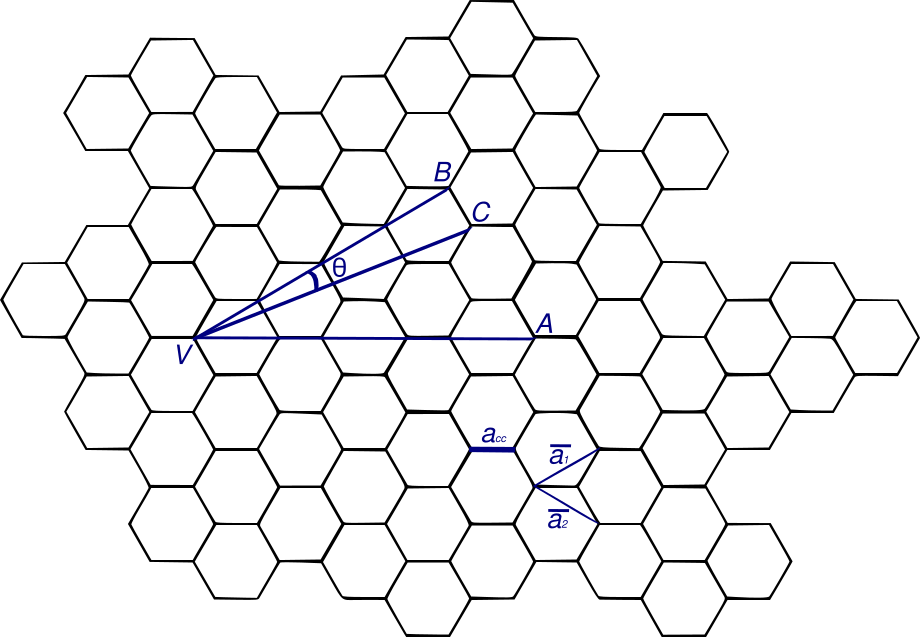
\includegraphics[width=0.7\textwidth]{images/panal1.png}
\caption{Caracterización de la quiralidad de un SWCNT a partir de la representación bidimensional de una lámina de grafeno que se enrolló para formar el nanotubo de carbono.}
\label{fig:quiralidad}
\end{figure}
En coordenadas cartesianas, el vector de quiralidad se expresa como:
\begin{align}
    \vec{C_h} &= \frac{a_{cc}\sqrt{3}}{2}(\sqrt{3}(m+n)\hat{i} + (n-m)\hat{j}) \\
     |\vec{C_h}| &= a_{cc}\sqrt{n^2 + m^2 + nm} 
\end{align}

El diámetro del nanotubo se puede calcular como \(d=|C_h|/\pi\). Además, a partir de las gráficas y ecuaciones, se puede deducir que:

\begin{align}
    \cos{\theta} = \frac{2n+m}{2\sqrt{n^2 + m^2 + nm}}
\end{align}

La notación (n, m) es fundamental para determinar la estructura y las propiedades de los SWNTs. Los nanotubos de carbono pueden tener una estructura armchair ($n = m$, $\theta=\frac{\pi}{6}$), zigzag ($m=0$, $\theta=0$) o chiral ($n \neq m$, $0<\theta<\frac{\pi}{6}$). Cada una de estas configuraciones tiene propiedades mecánicas únicas que se pueden simular mediante dinámica molecular \cite{avila2008molecular}.

La quiralidad también tiene un impacto significativo en las propiedades mecánicas de los SWNTs. Por ejemplo, la rigidez de Young y el módulo de cizallamiento de los SWNTs pueden depender del diámetro del tubo y de la quiralidad. En general, tanto la rigidez de Young como el módulo de cizallamiento aumentan con el diámetro del tubo para diámetros pequeños, y se vuelven insensibles al diámetro del tubo para diámetros más grandes. La quiralidad del tubo tiene un efecto insignificante en el módulo de cizallamiento para diámetros de tubo más grandes, pero puede tener algún efecto en la rigidez de Young para diámetros de tubo más pequeños \cite{li2003structural}.

Además, la quiralidad de los SWNTs también afecta a sus propiedades electrónicas. Los nanotubos de carbono pueden ser metálicos o semiconductores dependiendo de su quiralidad. Los nanotubos armchair son siempre metálicos, mientras que los nanotubos zigzag y chiral pueden ser metálicos o semiconductores dependiendo de si (n - m) es divisible por 3. Esta dependencia de las propiedades electrónicas de los SWNTs en su quiralidad tiene implicaciones importantes para su uso en aplicaciones de nanoelectrónica \cite{li2003structural}.

%%%%%%%%%%%%%%%%%%%%%%%%%%%%%%%%%%%%%%%%%%%%%%%%%%%%%%%%%%%%%%%%%%%%%%%%%%%%%%%%%%%%%%%%%%%%%%%%%%%%%%%%%%%%%%%%%%%%%%%
\section{Métodos de síntesis de SWNT y su influencia en las propiedades mecánicas}
%%%%%%%%%%%%%%%%%%%%%%%%%%%%%%%%%%%%%%%%%%%%%%%%%%%%%%%%%%%%%%%%%%%%%%%%%%%%%%%%%%%%%%%%%%%%%%%%%%%%%%%%%%%%%%%%%%%%
Los nanotubos de carbono de pared simple (SWCNT) son estructuras fascinantes que no se forman simplemente al enrollar una lámina de grafeno. En realidad, su síntesis requiere técnicas avanzadas como la deposición química de vapor asistida por plasma (PACVD). En este proceso, se coloca un sustrato en una cámara de reacción y se recubre con un catalizador metálico (fig. \ref{fig:PACVD}). Este catalizador es esencial para iniciar y dirigir el crecimiento de los SWCNT.

En el método PACVD, los átomos de carbono se disuelven en el catalizador metálico, formando un \textit{cluster} o agrupación de átomos de carbono y metal. A medida que más y más átomos de carbono se disuelven en el catalizador, eventualmente comienzan a formar una estructura de red hexagonal que se extiende desde el interior del \textit{cluster} y se fusiona por encima de la superficie del metal. Este es el inicio de la estructura de la tapa del nanotubo, un paso crucial en el crecimiento de un nanotubo de carbono \cite{shibuta2003molecular}.

\begin{figure}[h!]
    \centering
    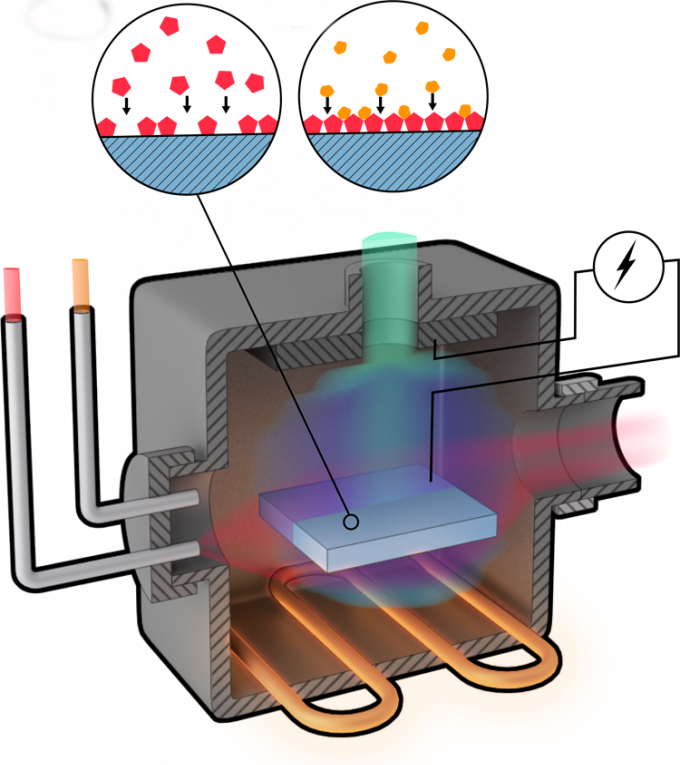
\includegraphics[width=0.4\textwidth]{images/figPACVD.png}
    \caption{PACVD: Recubrimiento asistido por plasma en vacío.}
    \label{fig:PACVD}
\end{figure}

La temperatura del sustrato, la presión del vapor, la concentración del catalizador y el voltaje aplicado entre los electrodos son factores clave que pueden influir en la distribución del diámetro de los SWCNT, así como en la formación de paredes simples o múltiples. Además, el tipo de gas utilizado, como el etanol, puede afectar la calidad y la cantidad de los SWCNT producidos \cite{kumar2010chemical}.

Además, la deposición química de vapor controlada por catalizador es uno de los métodos más directos para predefinir el diámetro o incluso la quiralidad de los SWCNT. Se han reportado numerosos estudios sobre la síntesis sensible a la quiralidad de los SWCNT utilizando una amplia variedad de catalizadores, incluyendo CoMo, FeCo, NiFe, Co, FeCu, Au, CoMn, Ni, Fe, CoPt, CoxMg1-xO, CoSO4, WCo y Mo2C. Estos catalizadores controladores de diámetro se utilizan para hacer crecer SWCNT a partir de diferentes fuentes de carbono, como monóxido de carbono (CO), metanol (CH3OH), metano (CH4) y etino (C2H2). Se ha observado una clara dependencia entre la presión del precursor de carbono y la selectividad de la quiralidad. En un rango de presión que varía de 2 a 18 bares, se observaron los rendimientos relativos predominantes de los SWCNT (6,5), (7,5) y (7,6). Esto demuestra que la química del precursor de carbono es una parte importante de los mecanismos de crecimiento de los SWCNT de (n,m) estrechamente agrupados \cite{kharlamova2023review}.


%%%%%%%%%%%%%%%%%%%%%%%%%%%%%%%%%%%%%%%%%%%%%%%%%%%%%%%%%%%%%%%%%%%%%%%%%%%%%%%%%%%%%%%%%%%%%%%%%%%%%%%%
\section{Potenciales interatómicos en simulaciones de dinámica molecular}
%%%%%%%%%%%%%%%%%%%%%%%%%%%%%%%%%%%%%%%%%%%%%%%%%%%%%%%%%%%%%%%%%%%%%%%%%%%%%%%%%%%%%%%%%%%%%%%%%%%%%%5%
Los potenciales interatómicos son funciones matemáticas que describen la energía de interacción entre los átomos en un sistema. Estos potenciales son fundamentales en las simulaciones de dinámica molecular (MD), ya que determinan cómo los átomos interactúan entre sí y, por lo tanto, cómo evoluciona el sistema con el tiempo.

En el caso de los nanotubos de carbono de pared simple (SWNT), los potenciales interatómicos deben ser capaces de describir correctamente las interacciones de carbono-carbono. Uno de los potenciales más utilizados para este propósito es el potencial de Tersoff-Brenner. Este potencial, desarrollado por Tersoff y luego modificado por Brenner, es un potencial de muchos cuerpos que tiene en cuenta no solo las interacciones entre pares de átomos, sino también las interacciones entre tres átomos. Esto es importante para los SWNT, ya que las propiedades de estos materiales están fuertemente influenciadas por los ángulos de enlace entre los átomos de carbono \cite{tersoff1988empirical, brenner2002second}.

El potencial de Tersoff-Brenner se obtuvo a partir de ajustes a los resultados de cálculos de estructura electrónica y a los datos experimentales. Este potencial ha demostrado ser muy efectivo para describir las propiedades mecánicas de los SWNT, incluyendo su resistencia a la tracción y su rigidez a la flexión \cite{tersoff1988empirical, brenner2002second}.

En las simulaciones de MD, también es importante considerar el número de átomos termostato, las técnicas de termostato, los pasos de tiempo y desplazamiento, y el número de pasos de relajación para alcanzar el equilibrio dinámico. Los átomos de termostato son átomos que se utilizan para controlar la temperatura del sistema. Estos átomos pueden intercambiar energía con el resto del sistema, lo que permite aumentar o disminuir la temperatura. Las técnicas de termostato son los métodos que se utilizan para controlar la temperatura, y pueden variar desde métodos simples que simplemente escalan las velocidades de los átomos, hasta métodos más sofisticados que simulan el acoplamiento del sistema a un baño térmico \cite{frenkel2001understanding}. Los pasos de tiempo y desplazamiento determinan cómo se actualizan las posiciones y velocidades de los átomos en cada paso de la simulación, y el número de pasos de relajación es el número de pasos que se deben realizar antes de que el sistema alcance el equilibrio dinámico \cite{frenkel2001understanding}.

Asimismo, el potencial REBO (Reactive Empirical Bond Order) es una extensión del potencial de Brenner que se utiliza para simular interacciones atómicas en sistemas de carbono. Este potencial se desarrolló para mejorar la descripción de la formación y ruptura de enlaces en sistemas de carbono durante las simulaciones de dinámica molecular.

El potencial REBO se basa en la idea de que la energía de un enlace entre dos átomos depende no solo de la distancia entre ellos, sino también del entorno atómico local. Específicamente, la energía del enlace depende del número y tipos de otros enlaces que cada átomo tiene. Por lo tanto, el potencial REBO puede describir con precisión la formación y ruptura de enlaces en sistemas de carbono, lo que es crucial para simular fenómenos como la deformación de los nanotubos de carbono.

En el contexto de la simulación de nanotubos de carbono de pared simple (SWCNT), el potencial REBO se utiliza para modelar las interacciones entre los átomos de carbono que forman el nanotubo. Este potencial permite simular con precisión cómo cambian las propiedades mecánicas del nanotubo a medida que se deforma, incluyendo la formación de cuellos de botella y la ruptura de enlaces.

%%%%%%%%%%%%%%%%%%%%%%%%%%%%%%%%%%%%%%%%%%%%%%%%%%%%%%%%%%%%%%%%%%%%%%%%%%%%%%%%%%%%%%%%%%%%%%%%%%%%%%5%
\section{Simulación de las propiedades mecánicas de los SWNT}
%%%%%%%%%%%%%%%%%%%%%%%%%%%%%%%%%%%%%%%%%%%%%%%%%%%%%%%%%%%%%%%%%%%%%%%%%%%%%%%%%%%%%%%%%%%%%%%%%%%%%%5%

El estudio de K. Mylvaganam \cite{mylvaganam2004important} emplea la dinámica molecular para investigar los cambios estructurales y las propiedades mecánicas de los nanotubos de carbono de armchair y zigzag. En este contexto, se utilizó el potencial REBO para simular la deformación de los SWNT bajo tensión. Los resultados de la simulación revelaron que el nanotubo comenzó a formar un cuello de botella a una tensión de alrededor de 0.39 para el nanotubo de armchair y 0.22 para el nanotubo de zigzag. Este fenómeno fue seguido por la formación de una cadena de un solo átomo, lo que indica la ruptura de los enlaces en el nanotubo. 

Este estudio identifica varios aspectos clave para la simulación de nanotubos de carbono, incluyendo la selección de potenciales interatómicos apropiados, el número de átomos termostato, las técnicas de termostato, los pasos de tiempo y desplazamiento, y el número de pasos de relajación para alcanzar el equilibrio dinámico. En particular, se concluye que la simulación utilizando el potencial de Tersoff-Brenner y el termostato de Berendsen con todos los átomos como átomos termostato (excepto los rígidos) y 50 pasos de relajación después de cada desplazamiento de 0.008 Å es un método más razonable y rentable \cite{mylvaganam2004important}. 

Además, se cuantifica que el módulo de Young y el coeficiente de Poisson del tubo armchair son 3.96 y 0.15 TPa, respectivamente, y los del tubo zigzag son 4.88 y 0.19 TPa, respectivamente. Se observó que el tubo armchair puede soportar una tensión más alta en comparación con el tubo zigzag. Bajo tensión, tanto los nanotubos armchair como los zigzag muestran el desenrollado de la cadena de carbono y una cadena de un solo átomo a una deformación de alrededor del 0.4.

Estos hallazgos proporcionan una guía valiosa para la realización de simulaciones de dinámica molecular para analizar los nanotubos de carbono y sus propiedades mecánicas. En particular, el potencial Tersoff y su aplicación a los sistemas de hidrocarburos, llamado potencial REBO, describen la ruptura/formación de enlaces utilizando un término de orden de enlace dependiente de la distancia y de muchos cuerpos \cite{irle2009milestones}. Estos avances en la simulación de dinámica molecular han permitido una comprensión más profunda de las propiedades mecánicas de los SWNT.

\begin{figure}[htbp]
  \centering
  \begin{subfigure}[b]{0.45\textwidth}
    \centering
    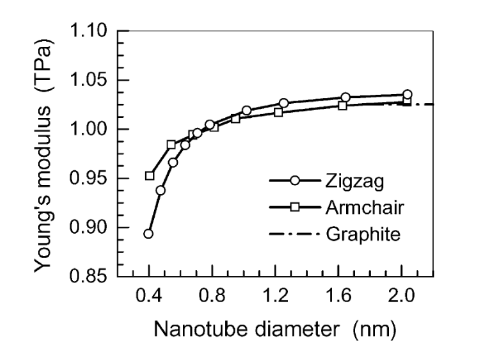
\includegraphics[width=\textwidth]{images/young-module.png}
    \caption{Representación gráfica del módulo de Young de los nanotubos de carbono (CNT) en función de su diámetro, ilustrando la relación entre la rigidez del material y su tamaño. Adaptado de \cite{li2003structural}}
    \label{fig:subfig1}
  \end{subfigure}
  \hfill
  \begin{subfigure}[b]{0.45\textwidth}
    \centering
    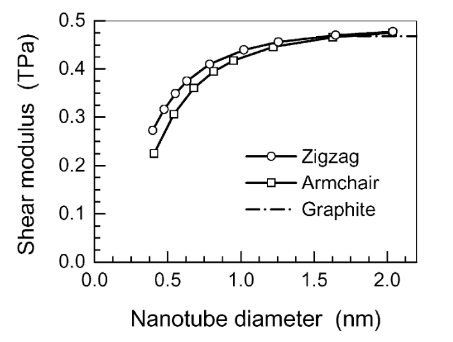
\includegraphics[width=\textwidth]{images/shear-module.png}
    \caption{Gráfico que muestra el módulo de corte de los nanotubos de carbono en función del diámetro del tubo, destacando cómo la resistencia al corte varía con el tamaño del nanotubo. Adaptado de \cite{li2003structural}}
    \label{fig:subfig2}
  \end{subfigure}
  \\
  \begin{subfigure}[b]{0.45\textwidth}
    \centering
    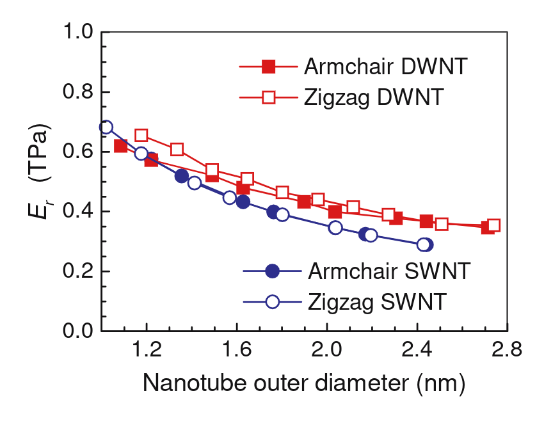
\includegraphics[width=\textwidth]{images/Radial module.png}
    \caption{Comparación del módulo radial entre los nanotubos de carbono de pared simple (SWCNT) y los de pared doble (DWNT), mostrando las diferencias en la rigidez radial entre estos dos tipos de nanotubos. Adaptado de \cite{li2006modeling}}
    \label{fig:subfig3}
  \end{subfigure}
  \hfill
  \begin{subfigure}[b]{0.45\textwidth}
    \centering
    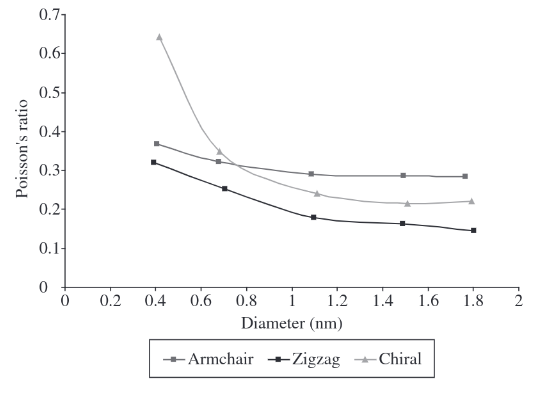
\includegraphics[width=\textwidth]{images/poisson-ratio.png}
    \caption{Variación del coeficiente de Poisson en función del diámetro de los nanotubos de carbono, ilustrando cómo la relación entre la deformación axial y radial cambia con el tamaño del nanotubo. Adaptado de \cite{avila2008molecular} }
    \label{fig:subfig4}
  \end{subfigure}
  \caption{Comparación de las propiedades mecánicas de los nanotubos de carbono en función de su diámetro.}
  \label{fig:subfiguras}
\end{figure} 

El estudio de Li y Chou \cite{li2006modeling} introduce un enfoque de mecánica estructural molecular para examinar las propiedades elásticas de los nanotubos de carbono. Este enfoque considera varias propiedades elásticas fundamentales, incluyendo el módulo de Young axial, el módulo de Young radial, el módulo de Young circunferencial y el módulo de cizallamiento. Para calcular estos módulos elásticos, se aplican diversas condiciones de carga, como tensión, torsión y presión hidrostática.

En este enfoque, un nanotubo de carbono de pared simple (SWCNT) se modela como una estructura de armazón espacial, donde los enlaces covalentes actúan como vigas y los átomos de carbono como nodos. Si se asume que los enlaces covalentes tienen una sección transversal redonda, solo se necesitan tres parámetros de rigidez: la resistencia a la tracción (EA), la rigidez flexural (EI) y la rigidez torsional (GJ). Estos parámetros están directamente relacionados con las constantes del campo de fuerza en la mecánica molecular, basándose en la equivalencia energética entre las energías potenciales locales y las energías de deformación elemental \cite{li2006modeling}:

\begin{align}
\frac{EA}{L}=k_r && \frac{EI}{L}=k_\theta && \frac{GJ}{L}=k_\tau
\end{align}

Donde $L$ denota la longitud del enlace, y $k_r$, $k_\theta$ y $k_\tau$ son las constantes del campo de fuerza en la mecánica molecular.

Las investigaciones han demostrado que los SWCNT poseen una alta resistencia a la tracción (EA), rigidez de flexión (EI) y resistencia a la torsión (GJ) \cite{mylvaganam2004important}. Como se puede observar en la Figura \ref{fig:subfig1}, el módulo de Young de los nanotubos de carbono (CNT) varía en función de su diámetro, lo que indica que la rigidez del material está influenciada por su tamaño. De manera similar, la Figura \ref{fig:subfig2} muestra cómo el módulo de corte de los nanotubos de carbono cambia con el diámetro del tubo.

Además, la Figura \ref{fig:subfig3} compara el módulo radial entre los nanotubos de carbono de pared simple (SWCNT) y los de pared doble (DWNT), mostrando las diferencias en la rigidez radial entre estos dos tipos de nanotubos. Por último, la Figura \ref{fig:subfig4} ilustra cómo varía el coeficiente de Poisson en función del diámetro de los nanotubos de carbono, lo que indica cómo la relación entre la deformación axial y radial cambia con el tamaño del nanotubo.

Los métodos de simulación utilizados para obtener estos resultados incluyen el método de Brenner, el potencial de Tersoff-Brenner y el potencial de ReaxFF, cada uno con sus propias ventajas y limitaciones \cite{mylvaganam2004important}. Estos métodos proporcionan una visión detallada de las propiedades mecánicas de los nanotubos de carbono y su dependencia del tamaño, lo que es crucial para su aplicación en nanotecnología y materiales avanzados.

%%%%%%%%%%%%%%%%%%%%%%%%%%%%%%%%%%%%%%%%%%%%%%%%%%%%%%%%%%%%%%%%%%%%%%%%%%%%%%%%%%%%%%%%%%%555%%%%%%
\section{Desafíos y oportunidades en la simulación de las propiedades mecánicas de los SWNT}
%%%%%%%%%%%%%%%%%%%%%%%%%%%%%%%%%%%%%%%%%%%%%%%%%%%%%%%%%%%%%%%%%%%%%%%%%%%%%%%%%%%%%%%%%%%%%%%%%%

La simulación de las propiedades mecánicas de los SWNT presenta varios desafíos. Estos incluyen la selección de potenciales interatómicos adecuados, el número de átomos termostato, las técnicas de termostato, los pasos de tiempo y desplazamiento, y el número de pasos de relajación para alcanzar el equilibrio dinámico. A pesar de estos desafíos, la dinámica molecular ofrece oportunidades para futuras investigaciones, como el desarrollo de nuevos métodos de simulación o la exploración de propiedades mecánicas no estudiadas \cite{mylvaganam2004important}.

El artículo de Li y Chou \cite{li2006modeling} menciona que las propiedades vibracionales de los nanotubos no se comprenden bien y que no hay informes sobre la modelización teórica de las propiedades dinámicas de los nanotubos de carbono mediante dinámica molecular. Además, el enfoque de la mecánica continua no puede aplicarse fácilmente para predecir las propiedades dinámicas de los nanotubos de carbono debido a la dificultad de distinguir la quiralidad del nanotubo y la incertidumbre en la definición del espesor de la pared del nanotubo. Sin embargo, se menciona que el enfoque de la mecánica estructural molecular puede ser útil para estudiar las propiedades térmicas de los nanotubos y los compuestos.

Uno de los desafíos asociados con la simulación de las propiedades mecánicas de los SWNT es la necesidad de modelos de interacción precisos. Se ha concluido que el uso de un potencial cuántico es esencial para una descripción cualitativamente correcta del comportamiento catalítico del cúmulo de metal, y que la formación de carburo no parece ser un requisito necesario para la nucleación y el crecimiento de los SWNT según las simulaciones de dinámica molecular química cuántica más recientes \cite{irle2009milestones}.

Por otro lado, las oportunidades para futuras investigaciones en este campo incluyen el desarrollo de nuevos métodos de simulación y la exploración de propiedades mecánicas no estudiadas. Por ejemplo, la dependencia de la temperatura de las tasas de crecimiento de SWNT catalizadas por hierro podría ser un área de investigación futura \cite{irle2009milestones}.

%%%%%%%%%%%%%%%%%%%%%%%%%%%%%%%%%%%%%%%%%%%%%%%%%%%%%%%%%%%%%%%%%%%%%%%%%%%%%%%%%%%%%%%%%%%%%%%%%%%%%%
\section{Conclusión}
%%%%%%%%%%%%%%%%%%%%%%%%%%%%%%%%%%%%%%%%%%%%%%%%%%%%%%%%%%%%%%%%%%%%%%%%%%%%%%%%%%%%%%%%%%%%%%%%%%%%%%%%

%Esta sección resumirá los puntos clave discutidos en el artículo y proporcionará una conclusión general.
%Resumen de los hallazgos más relevantes de cada estudio.
%Reflexión sobre la contribución del enfoque de simulación por dinámica molecular en el entendimiento del crecimiento y síntesis de SWNT.
%Posibles direcciones futuras de investigación y mejoras en los métodos de simulación

La quiralidad y las interacciones atómicas en los nanotubos de carbono de pared simple (SWNT) son factores determinantes en sus propiedades mecánicas, como la resistencia a la tensión, la rigidez de flexión y la resistencia a la torsión. La dinámica molecular, a pesar de los desafíos en su aplicación, como la selección de interacciones atómicas adecuadas y la gestión de la escala temporal y espacial, ha demostrado ser una herramienta esencial para analizar estas propiedades. Los métodos de simulación utilizados, incluyendo el método de Brenner, el potencial de Tersoff-Brenner y el potencial de ReaxFF, cada uno con sus propias ventajas y limitaciones, han proporcionado una visión valiosa en este campo \cite{avila2008molecular, mylvaganam2004important, irle2009milestones, li2006modeling}.

Mirando hacia el futuro, la necesidad de modelos de interacción precisos y la gestión de la escala temporal y espacial representan desafíos significativos en la simulación de las propiedades mecánicas de los SWNT. Sin embargo, también existen oportunidades para futuras investigaciones, como el desarrollo de nuevos métodos de simulación y la exploración de propiedades mecánicas no estudiadas. A medida que se desarrollen y perfeccionen nuevas técnicas de simulación, se espera que la comprensión de las propiedades mecánicas de los SWNT se profundice, abriendo la puerta a nuevas aplicaciones y tecnologías basadas en SWNT \cite{irle2009milestones}.

\printbibliography

\end{document} 
